% Options for packages loaded elsewhere
\PassOptionsToPackage{unicode}{hyperref}
\PassOptionsToPackage{hyphens}{url}
%
\documentclass[
]{article}
\usepackage{lmodern}
\usepackage{amssymb,amsmath}
\usepackage{ifxetex,ifluatex}
\ifnum 0\ifxetex 1\fi\ifluatex 1\fi=0 % if pdftex
  \usepackage[T1]{fontenc}
  \usepackage[utf8]{inputenc}
  \usepackage{textcomp} % provide euro and other symbols
\else % if luatex or xetex
  \usepackage{unicode-math}
  \defaultfontfeatures{Scale=MatchLowercase}
  \defaultfontfeatures[\rmfamily]{Ligatures=TeX,Scale=1}
\fi
% Use upquote if available, for straight quotes in verbatim environments
\IfFileExists{upquote.sty}{\usepackage{upquote}}{}
\IfFileExists{microtype.sty}{% use microtype if available
  \usepackage[]{microtype}
  \UseMicrotypeSet[protrusion]{basicmath} % disable protrusion for tt fonts
}{}
\makeatletter
\@ifundefined{KOMAClassName}{% if non-KOMA class
  \IfFileExists{parskip.sty}{%
    \usepackage{parskip}
  }{% else
    \setlength{\parindent}{0pt}
    \setlength{\parskip}{6pt plus 2pt minus 1pt}}
}{% if KOMA class
  \KOMAoptions{parskip=half}}
\makeatother
\usepackage{xcolor}
\IfFileExists{xurl.sty}{\usepackage{xurl}}{} % add URL line breaks if available
\IfFileExists{bookmark.sty}{\usepackage{bookmark}}{\usepackage{hyperref}}
\hypersetup{
  pdftitle={tp\_r\_compte\_rendu},
  pdfauthor={Florian Rascoussier},
  hidelinks,
  pdfcreator={LaTeX via pandoc}}
\urlstyle{same} % disable monospaced font for URLs
\usepackage[margin=1in]{geometry}
\usepackage{color}
\usepackage{fancyvrb}
\newcommand{\VerbBar}{|}
\newcommand{\VERB}{\Verb[commandchars=\\\{\}]}
\DefineVerbatimEnvironment{Highlighting}{Verbatim}{commandchars=\\\{\}}
% Add ',fontsize=\small' for more characters per line
\usepackage{framed}
\definecolor{shadecolor}{RGB}{248,248,248}
\newenvironment{Shaded}{\begin{snugshade}}{\end{snugshade}}
\newcommand{\AlertTok}[1]{\textcolor[rgb]{0.94,0.16,0.16}{#1}}
\newcommand{\AnnotationTok}[1]{\textcolor[rgb]{0.56,0.35,0.01}{\textbf{\textit{#1}}}}
\newcommand{\AttributeTok}[1]{\textcolor[rgb]{0.77,0.63,0.00}{#1}}
\newcommand{\BaseNTok}[1]{\textcolor[rgb]{0.00,0.00,0.81}{#1}}
\newcommand{\BuiltInTok}[1]{#1}
\newcommand{\CharTok}[1]{\textcolor[rgb]{0.31,0.60,0.02}{#1}}
\newcommand{\CommentTok}[1]{\textcolor[rgb]{0.56,0.35,0.01}{\textit{#1}}}
\newcommand{\CommentVarTok}[1]{\textcolor[rgb]{0.56,0.35,0.01}{\textbf{\textit{#1}}}}
\newcommand{\ConstantTok}[1]{\textcolor[rgb]{0.00,0.00,0.00}{#1}}
\newcommand{\ControlFlowTok}[1]{\textcolor[rgb]{0.13,0.29,0.53}{\textbf{#1}}}
\newcommand{\DataTypeTok}[1]{\textcolor[rgb]{0.13,0.29,0.53}{#1}}
\newcommand{\DecValTok}[1]{\textcolor[rgb]{0.00,0.00,0.81}{#1}}
\newcommand{\DocumentationTok}[1]{\textcolor[rgb]{0.56,0.35,0.01}{\textbf{\textit{#1}}}}
\newcommand{\ErrorTok}[1]{\textcolor[rgb]{0.64,0.00,0.00}{\textbf{#1}}}
\newcommand{\ExtensionTok}[1]{#1}
\newcommand{\FloatTok}[1]{\textcolor[rgb]{0.00,0.00,0.81}{#1}}
\newcommand{\FunctionTok}[1]{\textcolor[rgb]{0.00,0.00,0.00}{#1}}
\newcommand{\ImportTok}[1]{#1}
\newcommand{\InformationTok}[1]{\textcolor[rgb]{0.56,0.35,0.01}{\textbf{\textit{#1}}}}
\newcommand{\KeywordTok}[1]{\textcolor[rgb]{0.13,0.29,0.53}{\textbf{#1}}}
\newcommand{\NormalTok}[1]{#1}
\newcommand{\OperatorTok}[1]{\textcolor[rgb]{0.81,0.36,0.00}{\textbf{#1}}}
\newcommand{\OtherTok}[1]{\textcolor[rgb]{0.56,0.35,0.01}{#1}}
\newcommand{\PreprocessorTok}[1]{\textcolor[rgb]{0.56,0.35,0.01}{\textit{#1}}}
\newcommand{\RegionMarkerTok}[1]{#1}
\newcommand{\SpecialCharTok}[1]{\textcolor[rgb]{0.00,0.00,0.00}{#1}}
\newcommand{\SpecialStringTok}[1]{\textcolor[rgb]{0.31,0.60,0.02}{#1}}
\newcommand{\StringTok}[1]{\textcolor[rgb]{0.31,0.60,0.02}{#1}}
\newcommand{\VariableTok}[1]{\textcolor[rgb]{0.00,0.00,0.00}{#1}}
\newcommand{\VerbatimStringTok}[1]{\textcolor[rgb]{0.31,0.60,0.02}{#1}}
\newcommand{\WarningTok}[1]{\textcolor[rgb]{0.56,0.35,0.01}{\textbf{\textit{#1}}}}
\usepackage{graphicx,grffile}
\makeatletter
\def\maxwidth{\ifdim\Gin@nat@width>\linewidth\linewidth\else\Gin@nat@width\fi}
\def\maxheight{\ifdim\Gin@nat@height>\textheight\textheight\else\Gin@nat@height\fi}
\makeatother
% Scale images if necessary, so that they will not overflow the page
% margins by default, and it is still possible to overwrite the defaults
% using explicit options in \includegraphics[width, height, ...]{}
\setkeys{Gin}{width=\maxwidth,height=\maxheight,keepaspectratio}
% Set default figure placement to htbp
\makeatletter
\def\fps@figure{htbp}
\makeatother
\setlength{\emergencystretch}{3em} % prevent overfull lines
\providecommand{\tightlist}{%
  \setlength{\itemsep}{0pt}\setlength{\parskip}{0pt}}
\setcounter{secnumdepth}{-\maxdimen} % remove section numbering

\title{tp\_r\_compte\_rendu}
\author{Florian Rascoussier}
\date{1/12/2022}

\begin{document}
\maketitle

Voici le plan de ce qui sera fait dans le TP.

\hypertarget{visualisation-de-chemins}{%
\section{0. Visualisation de chemins}\label{visualisation-de-chemins}}

Le but de cette section est de vérifier que votre installation est
correcte, et de visualiser un problème du voyageur de commerce.

Lecture du fichier des villes :

\begin{Shaded}
\begin{Highlighting}[]
\CommentTok{# DonneesGPSvilles.csv contient les coordonnées GPS de 22 villes françaises}
\NormalTok{villes <-}\StringTok{ }\KeywordTok{read.csv}\NormalTok{(}\StringTok{'~/Documents/4if/s1/stats/tp_tsp/data/DonneesGPSvilles.csv'}\NormalTok{,}\DataTypeTok{header=}\OtherTok{TRUE}\NormalTok{,}\DataTypeTok{dec=}\StringTok{'.'}\NormalTok{,}\DataTypeTok{sep=}\StringTok{';'}\NormalTok{,}\DataTypeTok{quote=}\StringTok{"}\CharTok{\textbackslash{}"}\StringTok{"}\NormalTok{)}
\KeywordTok{str}\NormalTok{(villes)}
\end{Highlighting}
\end{Shaded}

\begin{verbatim}
## 'data.frame':    22 obs. of  5 variables:
##  $ EU_circo : chr  "Sud-Est" "Sud-Est" "Nord-Ouest" "Est" ...
##  $ region   : chr  "Rhône-Alpes" "Corse" "Picardie" "Franche-Comté" ...
##  $ ville    : chr  "Lyon" "Ajaccio" "Amiens" "Besançon" ...
##  $ latitude : num  45.7 41.9 49.9 47.2 44.8 ...
##  $ longitude: num  4.847 8.733 2.3 6.033 -0.567 ...
\end{verbatim}

Représentation des chemins par plus proches voisins et du chemin optimal
:

\begin{Shaded}
\begin{Highlighting}[]
\NormalTok{coord <-}\StringTok{ }\KeywordTok{cbind}\NormalTok{(villes}\OperatorTok{$}\NormalTok{longitude,villes}\OperatorTok{$}\NormalTok{latitude)}
\NormalTok{dist <-}\StringTok{ }\KeywordTok{distanceGPS}\NormalTok{(coord)}
\NormalTok{voisins <-}\StringTok{ }\KeywordTok{TSPnearest}\NormalTok{(dist)}

\NormalTok{pathOpt <-}\StringTok{ }\KeywordTok{c}\NormalTok{(}\DecValTok{1}\NormalTok{,}\DecValTok{8}\NormalTok{,}\DecValTok{9}\NormalTok{,}\DecValTok{4}\NormalTok{,}\DecValTok{21}\NormalTok{,}\DecValTok{13}\NormalTok{,}\DecValTok{7}\NormalTok{,}\DecValTok{10}\NormalTok{,}\DecValTok{3}\NormalTok{,}\DecValTok{17}\NormalTok{,}\DecValTok{16}\NormalTok{,}\DecValTok{20}\NormalTok{,}\DecValTok{6}\NormalTok{,}\DecValTok{19}\NormalTok{,}\DecValTok{15}\NormalTok{,}\DecValTok{18}\NormalTok{,}\DecValTok{11}\NormalTok{,}\DecValTok{5}\NormalTok{,}\DecValTok{22}\NormalTok{,}\DecValTok{14}\NormalTok{,}\DecValTok{12}\NormalTok{,}\DecValTok{2}\NormalTok{)}

\KeywordTok{par}\NormalTok{(}\DataTypeTok{mfrow=}\KeywordTok{c}\NormalTok{(}\DecValTok{1}\NormalTok{,}\DecValTok{2}\NormalTok{),}\DataTypeTok{mar=}\KeywordTok{c}\NormalTok{(}\DecValTok{1}\NormalTok{,}\DecValTok{1}\NormalTok{,}\DecValTok{2}\NormalTok{,}\DecValTok{1}\NormalTok{))}
\KeywordTok{plotTrace}\NormalTok{(coord[voisins}\OperatorTok{$}\NormalTok{chemin,], }\DataTypeTok{title=}\StringTok{'Plus proches voisins'}\NormalTok{)}
\KeywordTok{plotTrace}\NormalTok{(coord[pathOpt,], }\DataTypeTok{title=}\StringTok{'Chemin optimal'}\NormalTok{)}
\end{Highlighting}
\end{Shaded}

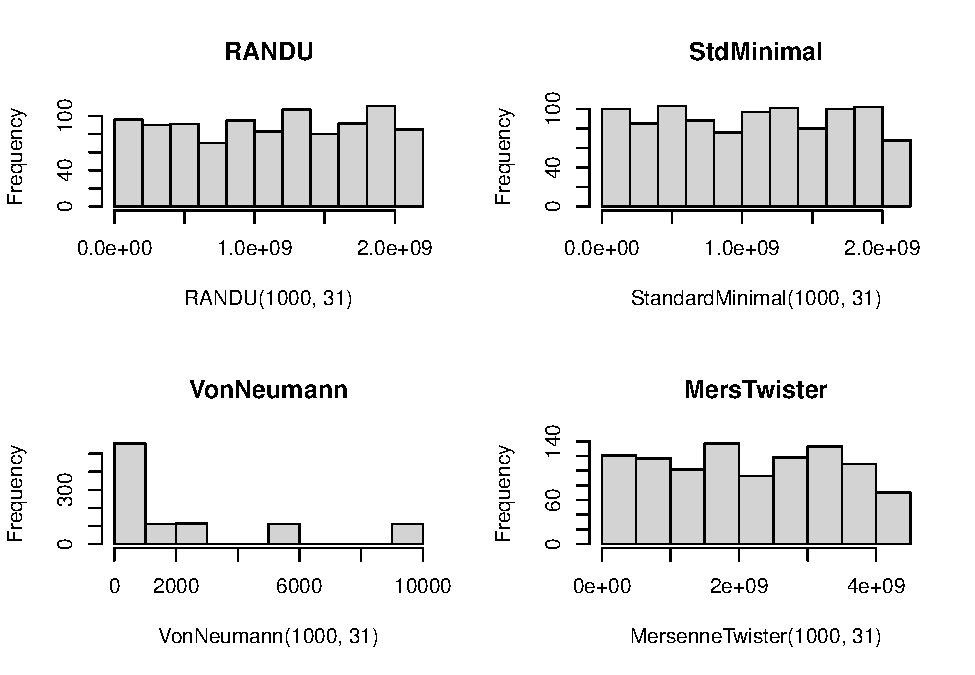
\includegraphics{compte_rendu_tp_tsp_files/figure-latex/unnamed-chunk-2-1.pdf}

Les longueurs des trajets (à vol d'oiseau) valent respectivement, pour
la \emph{méthode des plus proches voisins} :

\begin{verbatim}
## [1] 4303.568
\end{verbatim}

\begin{verbatim}
## [1] 4303.568
\end{verbatim}

et pour la \emph{méthode optimale} :

\begin{verbatim}
## [1] 3793.06
\end{verbatim}

\begin{verbatim}
## [1] 3793.06
\end{verbatim}

Ceci illustre bien l'intérêt d'un algorithme de voyageur de commerce.
Nous allons dans la suite étudier les performances de cet algorithme.
longueurs de di

\hypertarget{comparaison-dalgorithmes}{%
\section{1. Comparaison d'algorithmes}\label{comparaison-dalgorithmes}}

Comparaison de plusieurs algorithmes, donnant des solutions exactes et
approchées.

Nombre de sommets fixes et graphes ``identiques''.

\begin{Shaded}
\begin{Highlighting}[]
\CommentTok{# generate a new graph couts}
\NormalTok{      n <-}\StringTok{ }\DecValTok{10}
\NormalTok{sommets <-}\StringTok{ }\KeywordTok{data.frame}\NormalTok{(}\DataTypeTok{x =} \KeywordTok{runif}\NormalTok{(n), }\DataTypeTok{y =} \KeywordTok{runif}\NormalTok{(n)) }\CommentTok{# runif - get n points distributed along uniform law}
\NormalTok{  couts <-}\StringTok{ }\KeywordTok{distance}\NormalTok{(sommets)}
\end{Highlighting}
\end{Shaded}

\hypertarget{longueur-des-chemins}{%
\subsection{1.1. Longueur des chemins}\label{longueur-des-chemins}}

Comparaison des longueurs de différentes méthodes :

\begin{itemize}
\tightlist
\item
  boxplots
\end{itemize}

\begin{Shaded}
\begin{Highlighting}[]
\NormalTok{compare_methods <-}\StringTok{ }\KeywordTok{matrix}\NormalTok{(}\DecValTok{0}\NormalTok{,}\DecValTok{50}\NormalTok{,}\DecValTok{5}\NormalTok{)}
\NormalTok{method_names <-}\StringTok{ }\KeywordTok{c}\NormalTok{(}\StringTok{"repetitive_nn"}\NormalTok{, }\StringTok{"nearest_insertion"}\NormalTok{, }\StringTok{"two_opt"}\NormalTok{, }\StringTok{"nearest"}\NormalTok{, }\StringTok{"branch"}\NormalTok{)}
\KeywordTok{colnames}\NormalTok{(compare_methods) <-}\StringTok{ }\NormalTok{method_names}

\CommentTok{# create 50 seeds for the 50 repetitions}
\NormalTok{seeds <-}\StringTok{ }\KeywordTok{c}\NormalTok{(}\KeywordTok{seq}\NormalTok{(}\DataTypeTok{from=}\DecValTok{0}\NormalTok{,}\DataTypeTok{by=}\DecValTok{5}\NormalTok{,}\DataTypeTok{length=}\DecValTok{50}\NormalTok{))}
\NormalTok{methods_used_for_each_value <-}\StringTok{ }\KeywordTok{matrix}\NormalTok{(}\StringTok{""}\NormalTok{,}\DecValTok{50}\NormalTok{,}\DecValTok{5}\NormalTok{)}
\KeywordTok{colnames}\NormalTok{(methods_used_for_each_value) <-}\StringTok{ }\NormalTok{method_names}

\CommentTok{# compute 50 times the 5 methods}
\ControlFlowTok{for}\NormalTok{(i }\ControlFlowTok{in} \DecValTok{1}\OperatorTok{:}\DecValTok{50}\NormalTok{) \{}
  \CommentTok{# set current seed}
  \KeywordTok{set.seed}\NormalTok{(seeds[i])}
  
  \CommentTok{# generate a new graph}
\NormalTok{  n <-}\StringTok{ }\DecValTok{10}
\NormalTok{  sommets <-}\StringTok{ }\KeywordTok{data.frame}\NormalTok{(}\DataTypeTok{x =} \KeywordTok{runif}\NormalTok{(n), }\DataTypeTok{y =} \KeywordTok{runif}\NormalTok{(n)) }\CommentTok{# runif - get n points distributed along uniform law}
\NormalTok{  couts <-}\StringTok{ }\KeywordTok{distance}\NormalTok{(sommets) }\CommentTok{# the new graph}
  
  \CommentTok{# compute}
  \ControlFlowTok{for}\NormalTok{(j }\ControlFlowTok{in} \DecValTok{1}\OperatorTok{:}\NormalTok{(}\KeywordTok{length}\NormalTok{(method_names))) \{}
\NormalTok{    compare_methods[i, j] <-}\StringTok{ }\KeywordTok{TSPsolve}\NormalTok{(couts, method_names[j])}
\NormalTok{    methods_used_for_each_value[i,j] <-}\StringTok{ }\NormalTok{method_names[j]}
\NormalTok{  \}}
\NormalTok{\}}

\KeywordTok{boxplot}\NormalTok{(compare_methods)}
\end{Highlighting}
\end{Shaded}

\includegraphics{compte_rendu_tp_tsp_files/figure-latex/unnamed-chunk-6-1.pdf}
Les boxplots nous indiquent que ``branch'' est le meilleur (on le
savait), car les durées de transport sont les plus courtes. On peut se
demander si ``repetitive\_nn'' et ``branch'' sont similaires ou non.

\begin{itemize}
\tightlist
\item
  test entre `nearest' et `branch'
\end{itemize}

\begin{Shaded}
\begin{Highlighting}[]
\CommentTok{# H1 avec > -> alternative = greater}
\KeywordTok{pairwise.t.test}\NormalTok{(}\KeywordTok{cbind}\NormalTok{(compare_methods[,}\StringTok{"nearest"}\NormalTok{],compare_methods[,}\StringTok{"branch"}\NormalTok{]), }\KeywordTok{cbind}\NormalTok{(methods_used_for_each_value[,}\StringTok{"nearest"}\NormalTok{],methods_used_for_each_value[,}\StringTok{"branch"}\NormalTok{]), }\DataTypeTok{alternative =} \StringTok{"greater"}\NormalTok{, }\DataTypeTok{p.adjust.method =} \StringTok{"bonferroni"}\NormalTok{, }\DataTypeTok{paired =} \OtherTok{TRUE}\NormalTok{)}
\end{Highlighting}
\end{Shaded}

\begin{verbatim}
## 
##  Pairwise comparisons using paired t tests 
## 
## data:  cbind(compare_methods[, "nearest"], compare_methods[, "branch"]) and cbind(methods_used_for_each_value[, "nearest"], methods_used_for_each_value[, "branch"]) 
## 
##         branch 
## nearest 5.7e-11
## 
## P value adjustment method: bonferroni
\end{verbatim}

\begin{itemize}
\tightlist
\item
  tests 2 à 2
\end{itemize}

\begin{Shaded}
\begin{Highlighting}[]
\CommentTok{# H1 avec > -> alternative = greater}
\KeywordTok{pairwise.t.test}\NormalTok{(compare_methods, methods_used_for_each_value, }\DataTypeTok{alternative =} \StringTok{"greater"}\NormalTok{, }\DataTypeTok{p.adjust.method =} \StringTok{"bonferroni"}\NormalTok{, }\DataTypeTok{paired =} \OtherTok{TRUE}\NormalTok{)}
\end{Highlighting}
\end{Shaded}

\begin{verbatim}
## 
##  Pairwise comparisons using paired t tests 
## 
## data:  compare_methods and methods_used_for_each_value 
## 
##                   branch  nearest nearest_insertion repetitive_nn
## nearest           5.7e-10 -       -                 -            
## nearest_insertion 4.1e-09 1.00    -                 -            
## repetitive_nn     3.8e-05 1.00    1.00              -            
## two_opt           2.0e-09 1.00    0.37              2.4e-05      
## 
## P value adjustment method: bonferroni
\end{verbatim}

Quand la p-valeur est petite, on peut conclure que (H0) est fausse donc
que (H1) est vrai. Ici, rappel :

(H0) : moyenne method 1 == moyenne methode 2 (H1) : moyenne method 1 !=
moyenne methode 2

Donc ici, on peut déduire que ``branch'' a une moyenne différente des
autres, de même entre ``two\_opt'' et ``repetitive\_nn''. Pour le reste,
on ne peut rien dire.

Cela invalide notre hypothèse que ``branch'' et ``repetititve\_nn''
étaient similaires, puisqu'ils n'ont pas la même moyenne.

\hypertarget{temps-de-calcul}{%
\subsection{1.2. Temps de calcul}\label{temps-de-calcul}}

Comparaison des temps à l'aide du package microbenchmark.

Exemple d'application de microbenchmark :

\begin{Shaded}
\begin{Highlighting}[]
\KeywordTok{microbenchmark}\NormalTok{(}
  \KeywordTok{TSPsolve}\NormalTok{(couts, }\StringTok{"repetitive_nn"}\NormalTok{), }\KeywordTok{TSPsolve}\NormalTok{(couts, }\StringTok{"nearest_insertion"}\NormalTok{), }\KeywordTok{TSPsolve}\NormalTok{(couts, }\StringTok{"two_opt"}\NormalTok{), }\KeywordTok{TSPsolve}\NormalTok{(couts, }\StringTok{"nearest"}\NormalTok{), }\KeywordTok{TSPsolve}\NormalTok{(couts, }\StringTok{"branch"}\NormalTok{), }
  \DataTypeTok{times=}\DecValTok{20}\NormalTok{, }
  \DataTypeTok{setup=}\NormalTok{\{}
\NormalTok{    n <-}\StringTok{ }\DecValTok{10}
\NormalTok{    sommets <-}\StringTok{ }\KeywordTok{data.frame}\NormalTok{(}\DataTypeTok{x =} \KeywordTok{runif}\NormalTok{(n), }\DataTypeTok{y =} \KeywordTok{runif}\NormalTok{(n)) }\CommentTok{# runif - get n points distributed along uniform law}
\NormalTok{    couts <-}\StringTok{ }\KeywordTok{distance}\NormalTok{(sommets)}
\NormalTok{  \}}
\NormalTok{)}
\end{Highlighting}
\end{Shaded}

\begin{verbatim}
## Unit: microseconds
##                                  expr      min       lq      mean   median
##      TSPsolve(couts, "repetitive_nn") 8547.406 8960.842 9610.7460 9428.211
##  TSPsolve(couts, "nearest_insertion") 1437.373 1527.335 1617.3763 1619.316
##            TSPsolve(couts, "two_opt")  860.404  915.716 1036.5871  953.923
##            TSPsolve(couts, "nearest")   20.318   24.626   26.6389   25.898
##             TSPsolve(couts, "branch") 2027.387 3802.751 5949.3745 4989.866
##          uq       max neval  cld
##  10094.6820 11635.676    20    d
##   1680.0145  1896.051    20  b  
##   1014.6635  2023.342    20 ab  
##     27.9835    38.915    20 a   
##   7474.5070 13035.372    20   c
\end{verbatim}

``nearest'' is the fastest algorithm.

\hypertarget{etude-de-la-complexituxe9-de-lalgorithme-branch-and-bound}{%
\section{2. Etude de la complexité de l'algorithme Branch and
Bound}\label{etude-de-la-complexituxe9-de-lalgorithme-branch-and-bound}}

\hypertarget{comportement-par-rapport-au-nombre-de-sommets-premier-moduxe8le}{%
\subsection{2.1. Comportement par rapport au nombre de sommets : premier
modèle}\label{comportement-par-rapport-au-nombre-de-sommets-premier-moduxe8le}}

Récupération du temps sur 20 graphes pour différentes valeurs de \(n\).

Ajustement du modèle linéaire de \(\log(temps)^4\) en fonction de \(n\).

Analyse de la validité du modèle :

\begin{itemize}
\item
  pertinence des coefficients et du modèle,
\item
  étude des hypothèses sur les résidus.
\end{itemize}

\begin{Shaded}
\begin{Highlighting}[]
\NormalTok{nb_of_times <-}\StringTok{ }\DecValTok{10}
\NormalTok{seqn <-}\StringTok{ }\KeywordTok{c}\NormalTok{(}\KeywordTok{seq}\NormalTok{(}\DecValTok{4}\NormalTok{, }\DecValTok{20}\NormalTok{, }\DecValTok{1}\NormalTok{))}

\NormalTok{compute_time_per_n <-}\StringTok{ }\ControlFlowTok{function}\NormalTok{(n) \{}
  \KeywordTok{return}\NormalTok{(}
      \KeywordTok{microbenchmark}\NormalTok{(}
      \KeywordTok{TSPsolve}\NormalTok{(couts, }\DataTypeTok{method =} \StringTok{"branch"}\NormalTok{),}
      \DataTypeTok{times =}\NormalTok{ nb_of_times,}
      \DataTypeTok{setup =}\NormalTok{ \{}
\NormalTok{        couts <-}\StringTok{ }\KeywordTok{distance}\NormalTok{(}\KeywordTok{cbind}\NormalTok{(}\DataTypeTok{x =} \KeywordTok{runif}\NormalTok{(n), }\DataTypeTok{y =} \KeywordTok{runif}\NormalTok{(n)))}
\NormalTok{      \}}
\NormalTok{    )}\OperatorTok{$}\NormalTok{time}
\NormalTok{  )}
\NormalTok{\}}
\NormalTok{temps <-}\StringTok{ }\KeywordTok{t}\NormalTok{(}\KeywordTok{apply}\NormalTok{(}\DataTypeTok{X =} \KeywordTok{as.array}\NormalTok{(seqn), }\DataTypeTok{MARGIN =} \DecValTok{1}\NormalTok{, }\DataTypeTok{FUN =}\NormalTok{ compute_time_per_n)) }\CommentTok{# t() transpose}
\end{Highlighting}
\end{Shaded}

Représentation graphique de \(temps\) en fonction de \(n\) puis de sa
régression linéaire \(log(temps)^2\) en fonction de \(n\) :

\begin{Shaded}
\begin{Highlighting}[]
\KeywordTok{par}\NormalTok{(}\DataTypeTok{mflow=}\KeywordTok{c}\NormalTok{(}\DecValTok{1}\NormalTok{,}\DecValTok{2}\NormalTok{)) }\CommentTok{# 2 graphiques en 1 ligne}
\end{Highlighting}
\end{Shaded}

\begin{verbatim}
## Warning in par(mflow = c(1, 2)): "mflow" is not a graphical parameter
\end{verbatim}

\begin{Shaded}
\begin{Highlighting}[]
\KeywordTok{matplot}\NormalTok{(seqn, temps, }\DataTypeTok{xlab=}\StringTok{"n"}\NormalTok{, }\DataTypeTok{ylab=}\StringTok{"temps"}\NormalTok{, }\DataTypeTok{type =} \StringTok{"o"}\NormalTok{)}
\end{Highlighting}
\end{Shaded}

\includegraphics{compte_rendu_tp_tsp_files/figure-latex/unnamed-chunk-11-1.pdf}

\begin{Shaded}
\begin{Highlighting}[]
\KeywordTok{matplot}\NormalTok{(seqn, }\KeywordTok{log}\NormalTok{(temps)}\OperatorTok{^}\DecValTok{2}\NormalTok{, }\DataTypeTok{xlab=}\StringTok{"n"}\NormalTok{, }\DataTypeTok{ylab=}\KeywordTok{expression}\NormalTok{(}\KeywordTok{log}\NormalTok{(temps)}\OperatorTok{^}\DecValTok{2}\NormalTok{), }\DataTypeTok{type =} \StringTok{"o"}\NormalTok{)}
\end{Highlighting}
\end{Shaded}

\includegraphics{compte_rendu_tp_tsp_files/figure-latex/unnamed-chunk-11-2.pdf}
Ajustement du modèle lineaire de \(log(temps)^2\) en fonction de \(n\)
puis récupération des principales statistiques :

\begin{Shaded}
\begin{Highlighting}[]
\CommentTok{# ajustement du modèle lineaire de log(temps)^2}
\NormalTok{vect_temps <-}\StringTok{ }\KeywordTok{log}\NormalTok{(}\KeywordTok{as.vector}\NormalTok{(temps))}\OperatorTok{^}\DecValTok{2}
\NormalTok{vect_dim <-}\StringTok{ }\KeywordTok{rep}\NormalTok{(seqn, }\DataTypeTok{times=}\DecValTok{10}\NormalTok{)}
\NormalTok{temps.lm <-}\StringTok{ }\KeywordTok{lm}\NormalTok{(vect_temps}\OperatorTok{~}\NormalTok{vect_dim) }\CommentTok{# calcul des résidus}
\KeywordTok{summary}\NormalTok{(temps.lm)}
\end{Highlighting}
\end{Shaded}

\begin{verbatim}
## 
## Call:
## lm(formula = vect_temps ~ vect_dim)
## 
## Residuals:
##      Min       1Q   Median       3Q      Max 
## -104.889  -19.227    1.632   20.109  107.923 
## 
## Coefficients:
##             Estimate Std. Error t value Pr(>|t|)    
## (Intercept)  72.9016     5.8608   12.44   <2e-16 ***
## vect_dim     13.8685     0.4522   30.67   <2e-16 ***
## ---
## Signif. codes:  0 '***' 0.001 '**' 0.01 '*' 0.05 '.' 0.1 ' ' 1
## 
## Residual standard error: 28.88 on 168 degrees of freedom
## Multiple R-squared:  0.8485, Adjusted R-squared:  0.8476 
## F-statistic: 940.7 on 1 and 168 DF,  p-value: < 2.2e-16
\end{verbatim}

On obtient un résumé des résultats du calcul des résidus.

• \emph{Intercept} = constante • \emph{Estimate} = valeurs des
coefficients correspondant à chaque variable •
\emph{Pr(\textgreater\textbar t\textbar)} = p-valeur du test (H0)
coefficient=0 contre (H1) coefficient 6 = 0. `t' car c'est un test de
Student. Les * dans la marge servent à repérer les valeurs
significatives • Residual standard error = le σ̂ du cours · −y · k •
Multiple R-squared = le R 2 du cours en dimension 2, En plus grande
dimension, R 2 = kŷ ky · −y · k est le ratio entre la variance expliquée
par le modèle et la variance des données : si le ratio est proche de 1
cela signifie que les observations s'éloignent peu du modèle. •
F-statistic = test de Fisher de pertinence du modèle. Un modèle
pertinent est un modèle tel que R 2 N −K R 2 est significativement
supérieur à 0. F = 1−R 2 K−1 avec K le nombre de variables dans le
modèle (hors constante). La p-valeur donne la probabilité de se tromper
si on affirme que le modèle n'est pas pertinent. S'il n'y a qu'une seule
variable dans le modèle, tester (H0) coefficient=0 contre (H1)
coefficient 6 = 0 ou faire le test de pertinence global de Fisher sont
parfaitement équivalents.

plus la p-valeur est faible, plus le coef sert à quelque chose pour
l'influence sur la ``fitness'' du modèle.

Ici, p-value: \textless{} 2.2e-16 la p-valeur du modèle. Donc ici un
seul paramètre suffit largement.

Il faut vérifier les hypothèses sur les résidus. Il y en a 4 : • loi
normale • espérance nulle • variance constante • indépendance

Si l'une de ces hypothèse est remise en cause, alors le modèle n'est
plus valable (aucun des tests ci-dessus n'est valable et l'ajustement
pas les moindres carrés est également discutable).

L'étude de ces hypothèses se fait par • une étude graphique • des tests

Etude graphique

\begin{Shaded}
\begin{Highlighting}[]
\KeywordTok{par}\NormalTok{(}\DataTypeTok{mflow=}\KeywordTok{c}\NormalTok{(}\DecValTok{2}\NormalTok{,}\DecValTok{2}\NormalTok{)) }\CommentTok{# 4 graphiques}
\end{Highlighting}
\end{Shaded}

\begin{verbatim}
## Warning in par(mflow = c(2, 2)): "mflow" is not a graphical parameter
\end{verbatim}

\begin{Shaded}
\begin{Highlighting}[]
\KeywordTok{plot}\NormalTok{(temps.lm)}
\end{Highlighting}
\end{Shaded}

\includegraphics{compte_rendu_tp_tsp_files/figure-latex/unnamed-chunk-13-1.pdf}
\includegraphics{compte_rendu_tp_tsp_files/figure-latex/unnamed-chunk-13-2.pdf}
\includegraphics{compte_rendu_tp_tsp_files/figure-latex/unnamed-chunk-13-3.pdf}
\includegraphics{compte_rendu_tp_tsp_files/figure-latex/unnamed-chunk-13-4.pdf}
\emph{comment interpréter les résultats des graphiques ?}

• \textbf{Residuals vs Fitted} : -- Si on observe une tendance trop
marquée des points sur le graphique, cela signifie que l'espérance des
résidus n'est pas nulle, mais qu'elle est positive sur certaines
sections et négatives sur d'autres. Ce problème peut souvent être
corrigé avec un changement de variable. On reste assez ``tolérant'' sur
les tendances et il faut qu'elles soient marquées pour rejeter le
modèle.

-- Si on observe que le nuage de point s'écarte (forme de trompette) la
variance des résidus n'est pas constante. On dit que les résidus sont
hétéroscédastiques.

Ici, même si les points ne semble pas former une droite mais plutôt une
parabole, on peut quand même se dire que les observations graphiques ne
permettent pas de rejeter le modèle. C'est encore suffisament plat.
L'espérance des résidus est nulle.

• \textbf{Normal Q-Q} : Compare la distribution des résidus à une loi
normale. En abscisse, les quantiles empiriques des résidus et en
ordonnée les quantiles de la loi normale, avec estimation des paramètres
sur les résidus. Si les distribution sont identiques ou presque alors
l'ensemble des points sont sur la diagonale. Sinon on observera la
plupart du temps des deviation aux extremité ce qui sous-entend que les
queues de distribution sont différentes.

Ici, les points suivent relativement bien la droite donc pareil, c'est
bien aussi.

• \textbf{Scale location} : Idem que Residuals vs Fitted mais avec des
résidus normalisés.

Ici la droite est suffisament plate. Les résidus sont possiblement nuls.

• \textbf{Residuals vs Leverage} : Montre l'influence des echantillons
(plus un point est à droite et plus il en a). Si un point est un
outliers il apparaitra trés éloigné des autres et en dehors des bornes
par rapport à la distance de Cook. Ces bornes sont représentées par des
lignes rouge en pointillé. Il faut reprendre le modèle en enlevant les
points concernés s'il y en a pour vérifier qu'ils ne déterminent pas le
modèle à eux tout seuls. . .

Ici les points sont tous relativement proches de la courbe rouge, et
surtout ne dépassent aucune distance de Cook (en pointillé). On peut
donc être satisfait de l'influence des échantillons.

On peut faire un test du qui-2 ou de Shapiro pour vérifier les
hypothèses suivantes :

(H0) Les résidus suivent une loi normale (H1) Les résidus ne suivent pas
une loi normale

\begin{Shaded}
\begin{Highlighting}[]
\KeywordTok{shapiro.test}\NormalTok{(}\KeywordTok{residuals}\NormalTok{(temps.lm))}
\end{Highlighting}
\end{Shaded}

\begin{verbatim}
## 
##  Shapiro-Wilk normality test
## 
## data:  residuals(temps.lm)
## W = 0.98464, p-value = 0.0581
\end{verbatim}

Rappel : Dans chaque cas les tests doivent être appliqués sur les
résidus du modèle, et une p-valeur petite signifie un rejet de
l'hypothèse, donc du modèle de régression.

Ici la p-valeur est relativement grande, donc on peut peut rien
conclure, autrement dit, on ne peut pas réfuter (H0) et valider (H1) çàd
que on ne peut pas dire avec ce test, que les données ne suivent pas une
loi normale. ATTENTION : On ne peut cependant pas conclure pour autant
que les données suivent bien une loi normale !

\hypertarget{comportement-par-rapport-au-nombre-de-sommets-uxe9tude-du-comportement-moyen}{%
\subsection{2.2. Comportement par rapport au nombre de sommets : étude
du comportement
moyen}\label{comportement-par-rapport-au-nombre-de-sommets-uxe9tude-du-comportement-moyen}}

Récupération du temps moyen.

Ajustement du modèle linéaire de \(\log(temps.moy)^2\) en fonction de
\(n\).

Analyse de la validité du modèle :

\begin{itemize}
\item
  pertinence des coefficients et du modèle,
\item
  étude des hypothèses sur les résidus.
\end{itemize}

Affichage graphique de \(temps.moy\) et de sa régression linéaire :

\begin{Shaded}
\begin{Highlighting}[]
\NormalTok{temps.moy <-}\StringTok{ }\KeywordTok{rowMeans}\NormalTok{(temps) }\CommentTok{# on remplace nos lignes de 10 valeurs par la moyenne des ses valeurs}

\CommentTok{# affichage graphique de temps.moy et de sa linéarisation}
\KeywordTok{par}\NormalTok{(}\DataTypeTok{mflow=}\KeywordTok{c}\NormalTok{(}\DecValTok{1}\NormalTok{,}\DecValTok{2}\NormalTok{)) }\CommentTok{# 2 graphiques en 1 ligne}
\end{Highlighting}
\end{Shaded}

\begin{verbatim}
## Warning in par(mflow = c(1, 2)): "mflow" is not a graphical parameter
\end{verbatim}

\begin{Shaded}
\begin{Highlighting}[]
\KeywordTok{matplot}\NormalTok{(seqn, temps.moy, }\DataTypeTok{xlab=}\StringTok{"n"}\NormalTok{, }\DataTypeTok{ylab=}\StringTok{"temps.moy"}\NormalTok{, }\DataTypeTok{type =} \StringTok{"o"}\NormalTok{)}
\end{Highlighting}
\end{Shaded}

\includegraphics{compte_rendu_tp_tsp_files/figure-latex/unnamed-chunk-15-1.pdf}

\begin{Shaded}
\begin{Highlighting}[]
\KeywordTok{matplot}\NormalTok{(seqn, }\KeywordTok{log}\NormalTok{(temps.moy)}\OperatorTok{^}\DecValTok{2}\NormalTok{, }\DataTypeTok{xlab=}\StringTok{"n"}\NormalTok{, }\DataTypeTok{ylab=}\KeywordTok{expression}\NormalTok{(}\KeywordTok{log}\NormalTok{(temps)}\OperatorTok{^}\DecValTok{2}\NormalTok{), }\DataTypeTok{type =} \StringTok{"o"}\NormalTok{)}
\end{Highlighting}
\end{Shaded}

\includegraphics{compte_rendu_tp_tsp_files/figure-latex/unnamed-chunk-15-2.pdf}
Graphiquement, la régression linéaire à l'air correcte.

Ajustement du modèle de régression linéaire simple gaussien de
\(log(temps.moy)^2\) :

\begin{Shaded}
\begin{Highlighting}[]
\CommentTok{# ajustement du modèle de régression linéaire simple gaussien de log(temps.moy)^2}
\NormalTok{vect_temps_moy <-}\StringTok{ }\KeywordTok{log}\NormalTok{(}\KeywordTok{as.vector}\NormalTok{(temps.moy))}\OperatorTok{^}\DecValTok{2}
\CommentTok{# on a déjà vect_dim}
\NormalTok{temps.moy.lm <-}\StringTok{ }\KeywordTok{lm}\NormalTok{(vect_temps_moy}\OperatorTok{~}\NormalTok{seqn) }\CommentTok{# calcul des résidus}
\KeywordTok{summary}\NormalTok{(temps.moy.lm) }\CommentTok{# afficher un résumé du calcul des résidus}
\end{Highlighting}
\end{Shaded}

\begin{verbatim}
## 
## Call:
## lm(formula = vect_temps_moy ~ seqn)
## 
## Residuals:
##     Min      1Q  Median      3Q     Max 
## -34.079 -16.543   6.597  20.401  23.796 
## 
## Coefficients:
##             Estimate Std. Error t value Pr(>|t|)    
## (Intercept)   70.778     13.749   5.148 0.000119 ***
## seqn          14.616      1.061  13.779  6.4e-10 ***
## ---
## Signif. codes:  0 '***' 0.001 '**' 0.01 '*' 0.05 '.' 0.1 ' ' 1
## 
## Residual standard error: 21.43 on 15 degrees of freedom
## Multiple R-squared:  0.9268, Adjusted R-squared:  0.9219 
## F-statistic: 189.9 on 1 and 15 DF,  p-value: 6.397e-10
\end{verbatim}

p-valeur est très petite donc les coefs sont pertinents.

\begin{Shaded}
\begin{Highlighting}[]
\KeywordTok{par}\NormalTok{(}\DataTypeTok{mflow=}\KeywordTok{c}\NormalTok{(}\DecValTok{2}\NormalTok{,}\DecValTok{2}\NormalTok{)) }\CommentTok{# 4 graphiques}
\end{Highlighting}
\end{Shaded}

\begin{verbatim}
## Warning in par(mflow = c(2, 2)): "mflow" is not a graphical parameter
\end{verbatim}

\begin{Shaded}
\begin{Highlighting}[]
\KeywordTok{plot}\NormalTok{(temps.moy.lm)}
\end{Highlighting}
\end{Shaded}

\includegraphics{compte_rendu_tp_tsp_files/figure-latex/unnamed-chunk-17-1.pdf}
\includegraphics{compte_rendu_tp_tsp_files/figure-latex/unnamed-chunk-17-2.pdf}
\includegraphics{compte_rendu_tp_tsp_files/figure-latex/unnamed-chunk-17-3.pdf}
\includegraphics{compte_rendu_tp_tsp_files/figure-latex/unnamed-chunk-17-4.pdf}
On voit que Residuals vs Fitted et Scale-location sont pas vraiment
plats donc c'est l'hypothèse linéaire n'est pas géniale. Il faurait
faire une meilleur changement de variables.

Le résumé du calcul des résidus

\hypertarget{comportement-par-rapport-uxe0-la-structure-du-graphe}{%
\subsection{2.3. Comportement par rapport à la structure du
graphe}\label{comportement-par-rapport-uxe0-la-structure-du-graphe}}

Lecture du fichier `DonneesTSP.csv'.

Ajustement du modèle linéaire de \(\log(temps.moy)\) en fonction de
toutes les variables présentes. Modèle sans constante.

Mise en \oe uvre d'une sélection de variables pour ne garder que les
variables pertinentes.

Analyse de la validité du modèle :

\begin{itemize}
\item
  pertinence des coefficients et du modèle,
\item
  étude des hypothèses sur les résidus.
\end{itemize}

\end{document}
